\documentclass{article}
\newenvironment{standalone}{\begin{preview}}{\end{preview}}
\usepackage{../includes}
\externaldocument{modelo}

\begin{document}
\begin{standalone}
  \section{Implementación}

  \subsection{Componentes}

  Para la implementación del emulador de arreglo de antenas utilizamos dos componentes: un microcontrolador y un sintetizador digital directo.

  El microcontrolador elegido es un STM32F103 de ST dentro de la placa de desarrollo Blue-Pill que puede verse en la \cref{fig:blue-pill}.
  El STM32F103 es un microcontrolador de 32-bit que trabaja a una frecuencia máxima de 72MHz, tiene una memoria flash de 64 o 128KB y entre otras características, cuenta con siete temporizadores e interfaces de comunicación SPI, I2C, USART, CAN y USB \cite{STM32F103_datasheet}.

  \begin{figure}[!htbp]
    \centering
    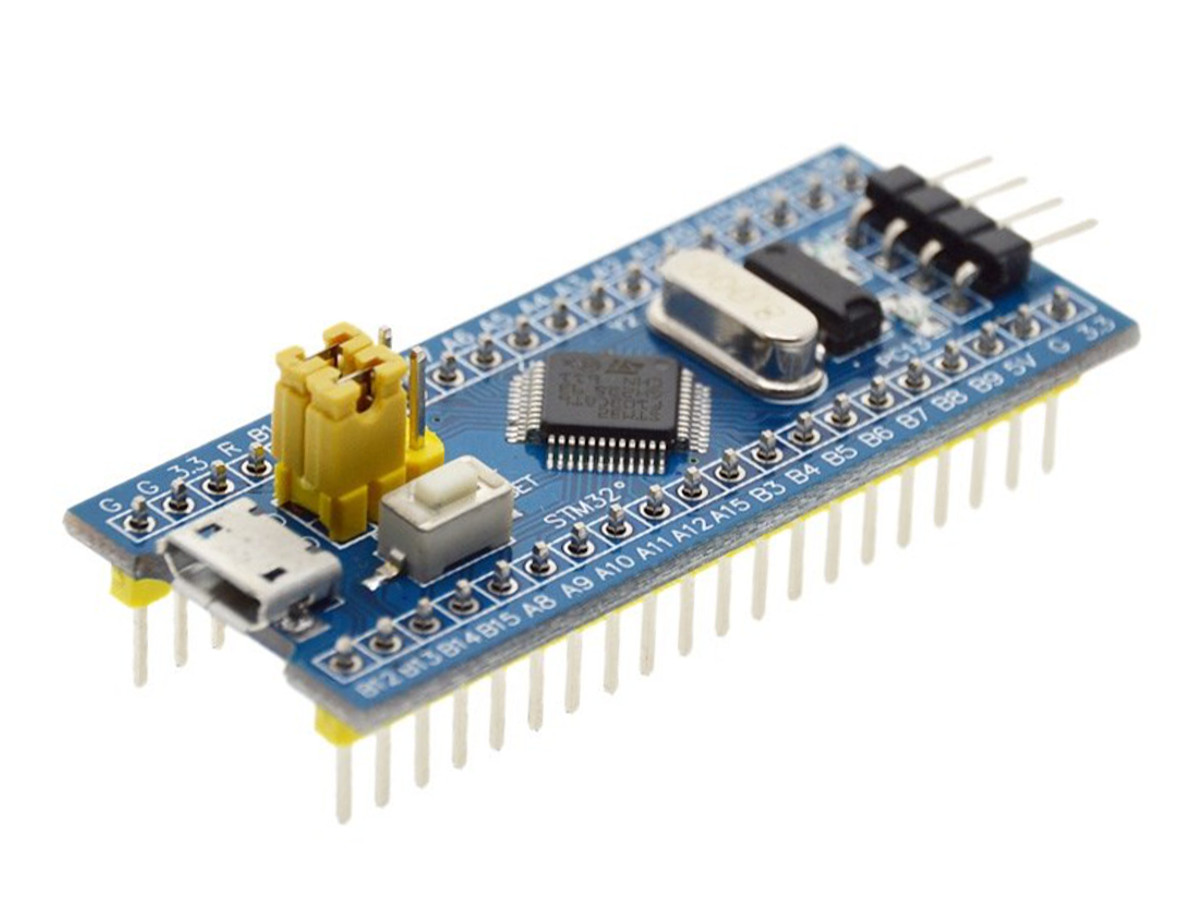
\includegraphics[width=\linewidth, height=50mm, keepaspectratio]{../images/bluepill-stm32.jpg}
    \caption{Placa de desarrollo Blue-Pill con un microcontrolador STM32F103.}
    \label{fig:blue-pill}
  \end{figure}

  Para el sintetizador digital directo, se cuenta con una placa de desarrollo del AD9959 de la empresa Analog Devices como la de la \cref{fig:ad9959}.
  El AD9959 es un sintetizador digital directo de 4-canales que trabaja a una frecuencia máxima de 500 MHz y cuenta con conversores digital-analógico de 10-bits y comunicación SPI \cite{ad9959_datasheet}.

  \begin{figure}[!htbp]
    \centering
    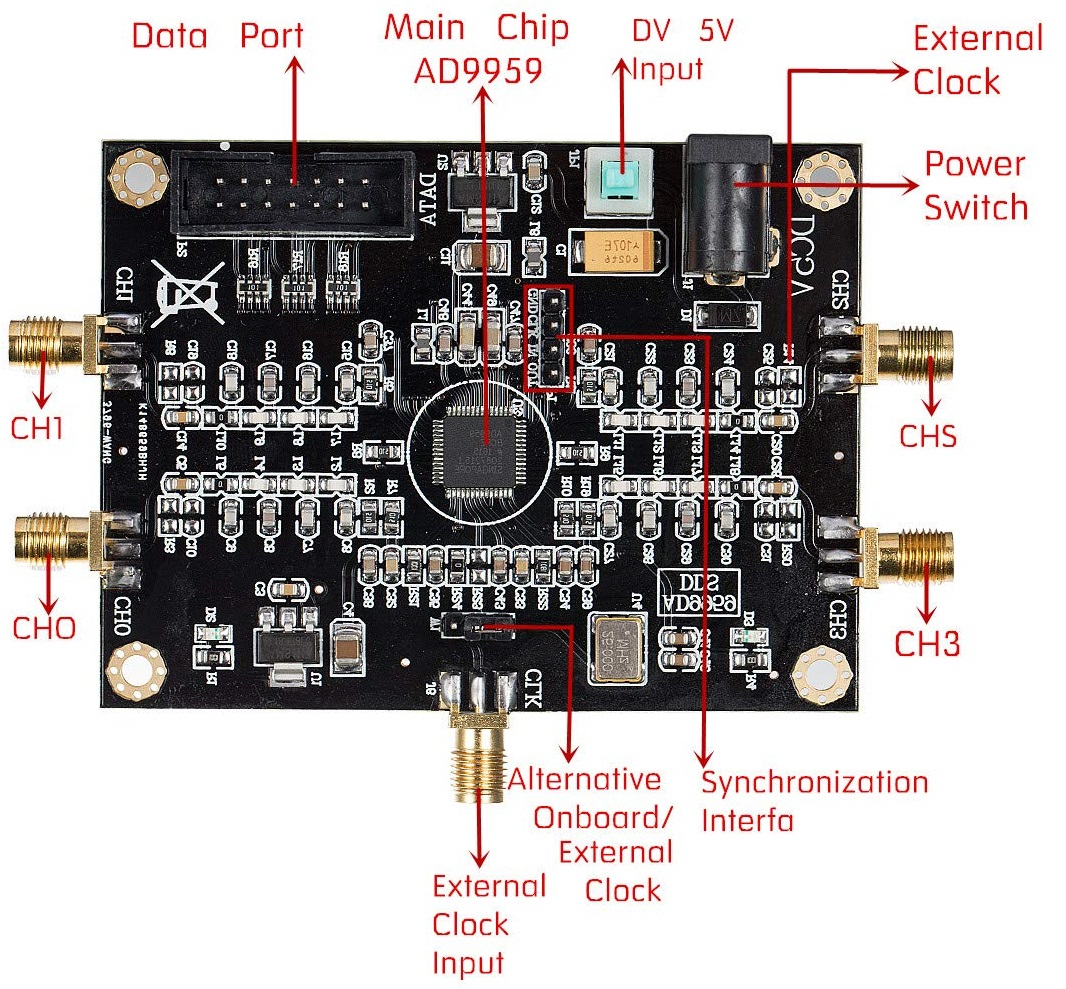
\includegraphics[width=\linewidth, height=60mm, keepaspectratio]{../images/ad9959.jpg}
    \caption{Placa de desarrollo del sintetizador digital AD9959.}
    \label{fig:ad9959}
  \end{figure}

  \subsection{Comunicación y conexiones}

  La placa de desarrollo del A9959 tiene 14 pines de entrada y salida y un jumper.
  Conectamos los pines de entrada y salida al microcontrolador como se muestra en la \cref{fig:conexiones}.

  \begin{figure}[!htbp]
    \centering
    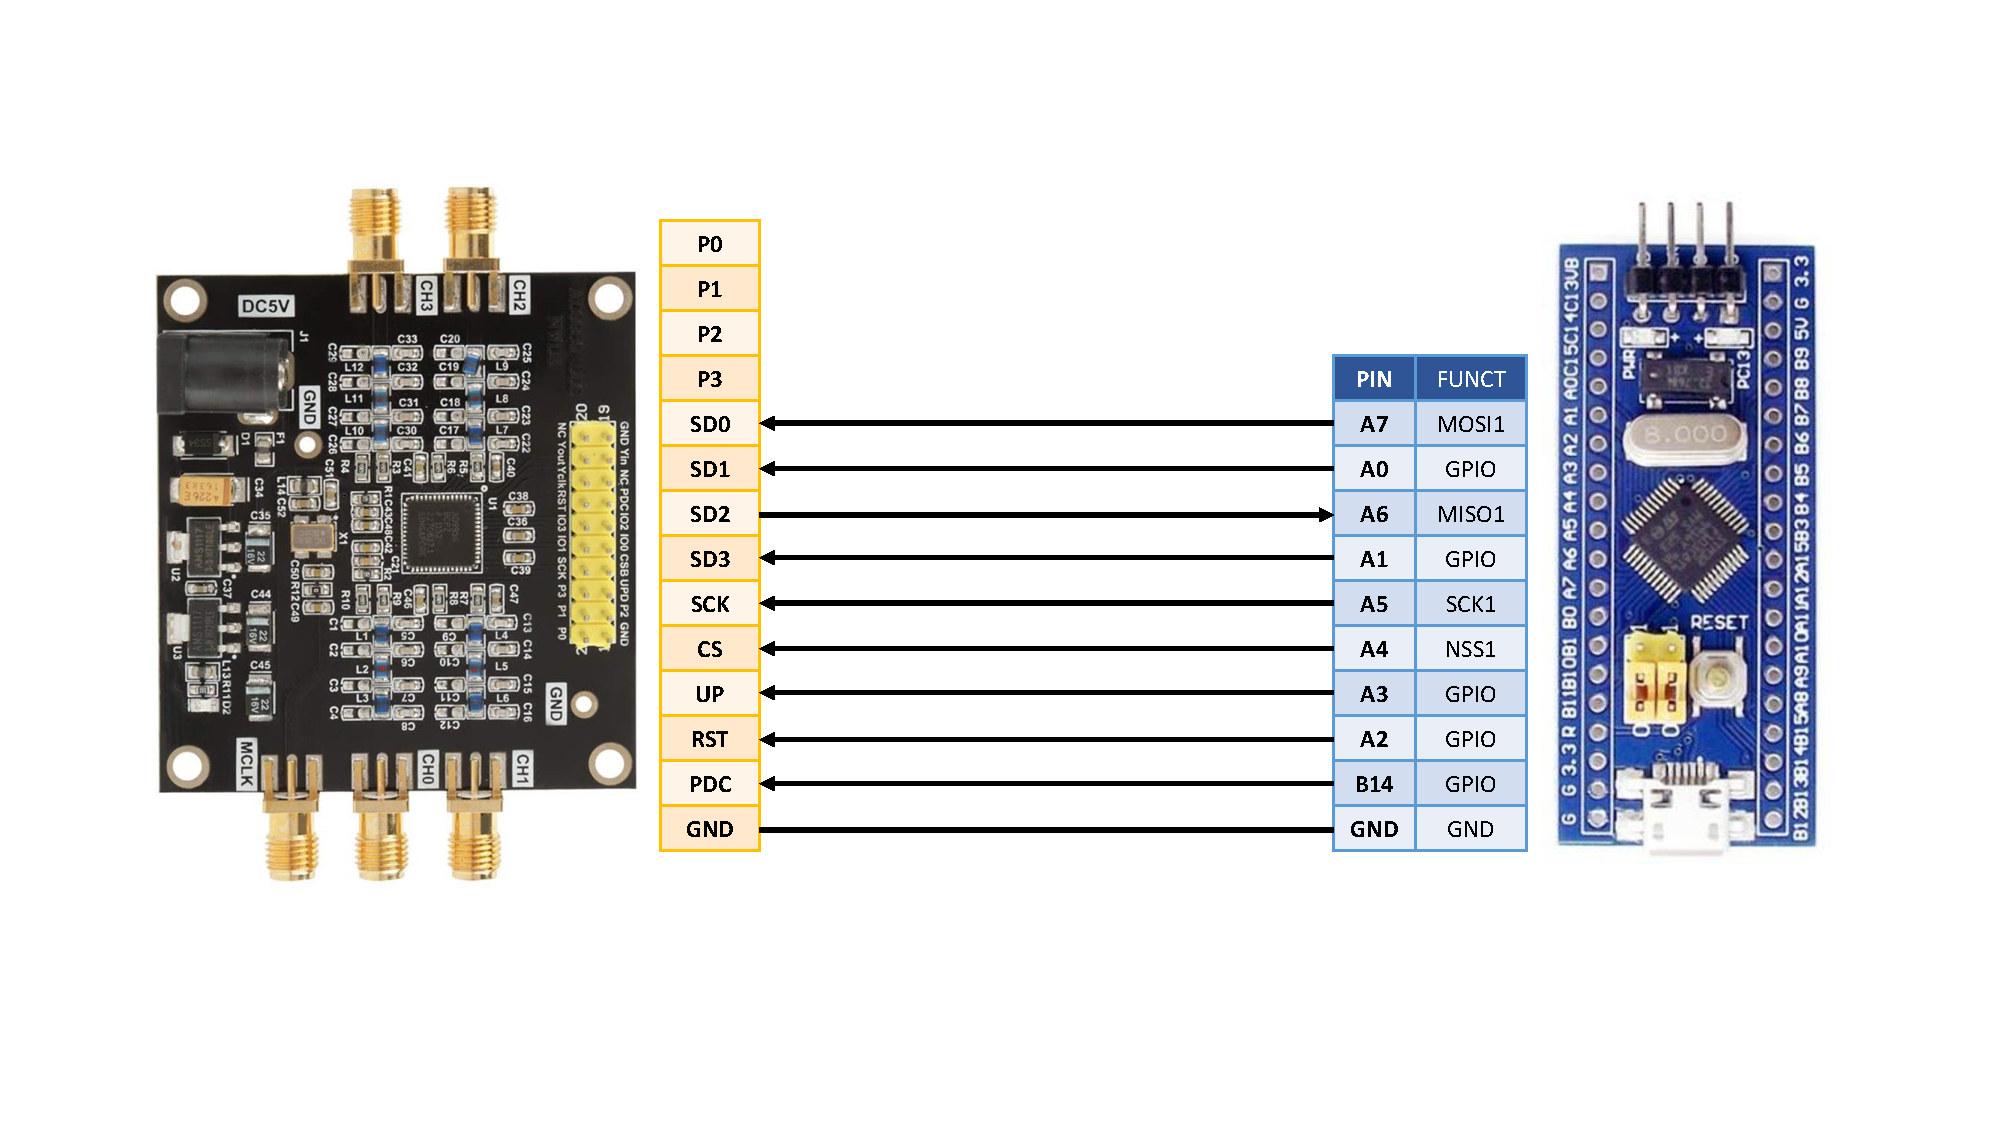
\includegraphics[trim=40pt 100pt 40pt 100pt, clip, width=\linewidth, height=60mm, keepaspectratio]{../images/conexiones.pdf}
    \caption{Conexiones entre microcontrolador y DDS.}
    \label{fig:conexiones}
  \end{figure}

  Como se mencionó, el AD9959 se comunica a través de una interfaz SPI.
  Existen cuatro modos de comunicación programables para este dispositivo: un bit serie con dos cables, un bit serie con tres cables, dos bits serie y cuatro bits serie.
  Uno, dos y cuatro bits serie hacen referencia a la cantidad de bits que se transmiten en cada flanco ascendente del reloj.
  Para el modo de un bit serie, la transmisión y recepción puede hacerse por un canal bidireccional (dos cables) o dos canales unidireccionales (tres cables).
  Los modos de dos y cuatro bits usan canales bidireccionales.
  En nuestra implementación, usamos el modo un bit serie con tres cables por ser el estándar más utilizado para comunicaciones SPI.

  Los pines SDIO\_0 a SDIO\_3 se usan para transmisión y recepción de datos y, si el modo de comunicación elegido deja algún pin libre, para realizar operaciones de \textit{ramp-up} y \textit{ramp-down} (RD/RD) y/o para sincronizar múltiples sintetizadores digitales directos.
  Para el modo elegido, el pin SDIO\_0 funciona como entrada al sintetizador, es decir, \textit{Master-Out Slave-In} (MOSI), y el pin SDIO\_2, como salida, es decir, \textit{Master-In Slave-Out} (MISO).
  Conectamos entonces el pin SDIO\_0 del DDS al pin A7 del microcontrolador que corresponde a la función MOSI de la interfaz SPI1 (MOSI1) y el pin SDIO\_2 al A6 (MISO1).
  Como para este prototipo no utilizaremos las funciones secundarias de los pines SDIO\_X, los conectamos a pines GPIO configurados como salidas en 0.

  El protocolo SPI también necesita dos pines adicionales: una línea de reloj que permite sincronizar la comunicación y un pin de selección para activar y desactivar la comunicación al dispositivo.
  Conectamos los pines de relok SCLK y de selección \textoverline{CS} del sintetizador a los pines A5 (SCK1) y A4 (NSS1) del microcontrolador.

  El pin IO\_UPDATE del AD9959 tiene como función transferir los datos recibidos de un buffer a los verdaderos registros.
  Esto produce que los cambios efectuados en el dispositivo se apliquen simulténeamente con el flanco ascendente del pin IO\_UPDATE.
  Conectamos este pin a A3 como salida digital del microcontrolador.

  El pin MASTER\_RESET es una entrada digital que, cuando recibe un 1, reinicia los registros del sintetizador a sus valores por defecto.
  Conectamos este pin a A2 como salida digital del microcontrolador.

  El pin PWR\_DWN\_CTL controla el modo de ahorro de energía.
  Cuando esta entrada recibe un 1, se activa el modo de ahorro de energía.
  Como estaremos constatemente usando el sintetizador, conectamos este pin al GPIO B14 del microcontrolador configurado como salida en 0.

  Los pines P0 a P3 del AD9959 se usan para modulación.
  Como no utilizaremos esta funcionalidad, podemos dejar estos pines flotando.

  Necesitamos además que el sintetizador y el microcontrolador tengan una tierra común.
  Para esto, conectamos los pines GND de ambos dispositivos.

  Por último, el jumper que tiene la placa de desarrollo del AD9959 controla la entrada de reloj de referencia del sintetizador.
  Se puede elegir entre una entrada externa de reloj o un cristal de 25 MHz que ya viene en la placa.
  Por simplicidad, elegimos la última opción.

  \todo[inline]{Agregar algo sobre los pines para sincronizar varios DDS}

  \subsection{Configuración inicial de registros}

  El sintetizador AD9959 posee una cantidad considerable de registros que controlan las distintas funciones del dispositivo.
  Pero para nuestro prototipo sólo necesitaremos modificar dos registros en la configuración inicial como se explica a continuación.

  El registro \textit{Channel Selection Register} (CSR) de la dirección 0x00:
  \begin{table}[!htbp]
    \centering
    \begin{tabular}{|c|c|c|c|c|c|c|c|}
    \hline
    \rowcolor[HTML]{EFEFEF}
    Bit7 & Bit6 & Bit5 & Bit4 & Bit3 & Bit2 & Bit1 & Bit0 \\ \hline
    X    & X    & X    & X    & 0    & 0    & 1    & 0    \\ \hline
    \end{tabular}
  \end{table}

  Los bits 7 a 4 seleccionan los canales a los que se le aplican los cambios.
  En la configuración inicial no es necesario seleccionar ningún canal.
  El bit 3 debe ser 0.
  Los bits 2 y 1 configuran el modo de comunicación.
  El valor b01 selecciona el modo de un bit serie con tres cables.
  El bit 0 en 0 determina que el formato de los datos es bit más significativo primero (MSB).

  El registro \textit{Function Register 1} (FR1) de la dirección 0x01:
  \begin{table}[!htbp]
    \centering
    \begin{tabular}{|c|c|c|c|c|c|c|c|}
    \hline
    \rowcolor[HTML]{EFEFEF}
    Bit23 & Bit22 & Bit21 & Bit20 & Bit19 & Bit18 & Bit17 & Bit16 \\ \hline
    1     & 1     & 0     & 1     & 0     & 0     & 0     & 0     \\ \hline
    \rowcolor[HTML]{EFEFEF}
    Bit15 & Bit14 & Bit13 & Bit12 & Bit11 & Bit10 & Bit9  & Bit8  \\ \hline
    0     & 0     & 0     & 0     & 0     & 0     & 0     & 0     \\ \hline
    \rowcolor[HTML]{EFEFEF}
    Bit7  & Bit6  & Bit5  & Bit4  & Bit3  & Bit2  & Bit1  & Bit0  \\ \hline
    0     & 0     & 0     & 0     & 0     & 0     & 0     & 0     \\ \hline
    \end{tabular}
  \end{table}

  Este registro nos permite, principalmente, configurar la frecuencia del sistema.
  Los bits 22:18 determinan la relación de división del PLL.
  Este valor, de 4 a 20, multiplica la frecuencia del reloj de entrada.
  Asignamos el valor 20 = 0b10100 para obtener la máxima frecuencia $20 \times 25 \ \si{\mega\hertz} = 500 \ \si{\mega\hertz}$.

  El bit 23 debe ser 1 para frecuencias del sistema superiores a 255 MHz.
  Los demás bits no son de relevancia para nuestra aplicación y los dejamos en 0.

  \subsection{Control de las señales generadas}

  Una vez que hemos realizado la configuración inicial de registros, podemos comenzar con la emulación propiamente dicha.

  Configuramos el Timer1 del microcontrolador para realizar una interrupción cada milisegundo, es decir, con una velocidad de 1 kHz.
  En cada interrupción se calcula la posición del sátelite y en base a ello, la frecuencia, amplitud y fase de las señales recibidas por los elementos del arreglo de antena como se describió en el \cref{sec:modelo-senales}.
  Luego, se escriben los registros necesarios para obtener estas señales en los canales del sintetizador como explicaremos a continuación.

  Primero, debemos seleccionar el canal que queremos modificar.
  Recordemos que para ello se deben escribir los bits 7 a 4 del registro CSR, dirección 0x00.
  Un 1 activa el canal y un 0 lo desactiva.
  El bit 7 controla el canal 3, el bit 6, el canal 2, el bit 5, el canal 1 y el bit 4, el canal 0.
  Al escribir este registro, debemos tener cuidado en respetar los valores del resto de los bits que asignamos para la configuración deseada.

  Por un lado, para asignar la frecuencia, escribimos el registro de 4-bytes \textit{Channel Frequency Tuning Word 0} (CFTW0), dirección 0x04.
  El valor de la palabra de 32-bits a asignar, \textit{Frequency Tuning Word} (FTW), está dada por
  \begin{equation}
    FTW = \frac{ f_{out} }{ f_s } \times 2^{32},
  \end{equation}
  siendo $f_{out} \ [\si{\hertz}]$ la frecuencia de salida deseada y $f_s \ [\si{\hertz}]$, la frecuencia del sistema (teniendo en cuenta la división del PLL).
  Como sabemos por la teoría de Nyquist, $f_{out} \leq f_s / 2$.

  Por otro lado, para asignar la fase, escribimos el registro de 2-bytes \textit{Channel Phase Offset Word 0} (CPOW0), dirección 0x05.
  El valor de la palabra de 14-bits, \textit{Phase Offset Word} (POW), a asignar en los bits 13 a 0, está dada por
  \begin{equation}
    POW = \frac{\phi_{out}}{360} \times 2^{14},
  \end{equation}
  siendo $0\degree \leq \phi_{out} < 360\degree$ la fase de salida deseada.
  Los bits 15 y 14 pueden tomar cualquier valor.

  Por último, para asignar la amplitud, escribimos el registro de 3-bytes \textit{Amplitude Control Register} (ACR), dirección 0x06.
  El valor de la palabra de 10-bits, \textit{Amplitude Scale Factor} (ASC), a asignar en los bits 9 a 0, está dada por
  \begin{equation}
    ASC = a_{out} \times \left( 2^{10} - 1 \right),
  \end{equation}
  siendo $0 \leq a_{out} \leq 1$ la amplitud de salida normalizada.
  Los bits 23 a 10 definen otros parámetros de la amplitud que no utilizaremos para nuestro prototipo, por lo que los dejamos en 0.

\end{standalone}
\end{document}
